\subsection{\progcl{}}\label{subsec:progcl}

\citeauthor{progcl_2022} propose an approach to mine negative samples for \ac{cl} on graphs called \progcl{}. 
As a motivation, the authors compare the similarity between the anchor and true negative samples to the similarity between the anchor and \acp{fn} 
across multiple datasets for both conventional \ac{cl} and \ac{gcl}.
The resulting distributions shown in \autoref{fig:sim_t_f_neg_image_graph} 
indicate that for \ac{gcl} most highly similar negative samples are \acp{fn}, while for \ac{cl} there is not a clear trend for \ac{cl}.
Moreover, the authors found that both the \ac{tn} and \ac{fn} distributions are modeled best by a beta mixture model %\ac{bmm} 
since it is able to fit the skewed empirical distribution.
The distribution is fitted using the \ac{em} algorithm on a subset of samples for a reduction of computational costs.

\begin{figure}%
    \centering
    \subfloat[\centering CIFAR-10 (Image)]
    {{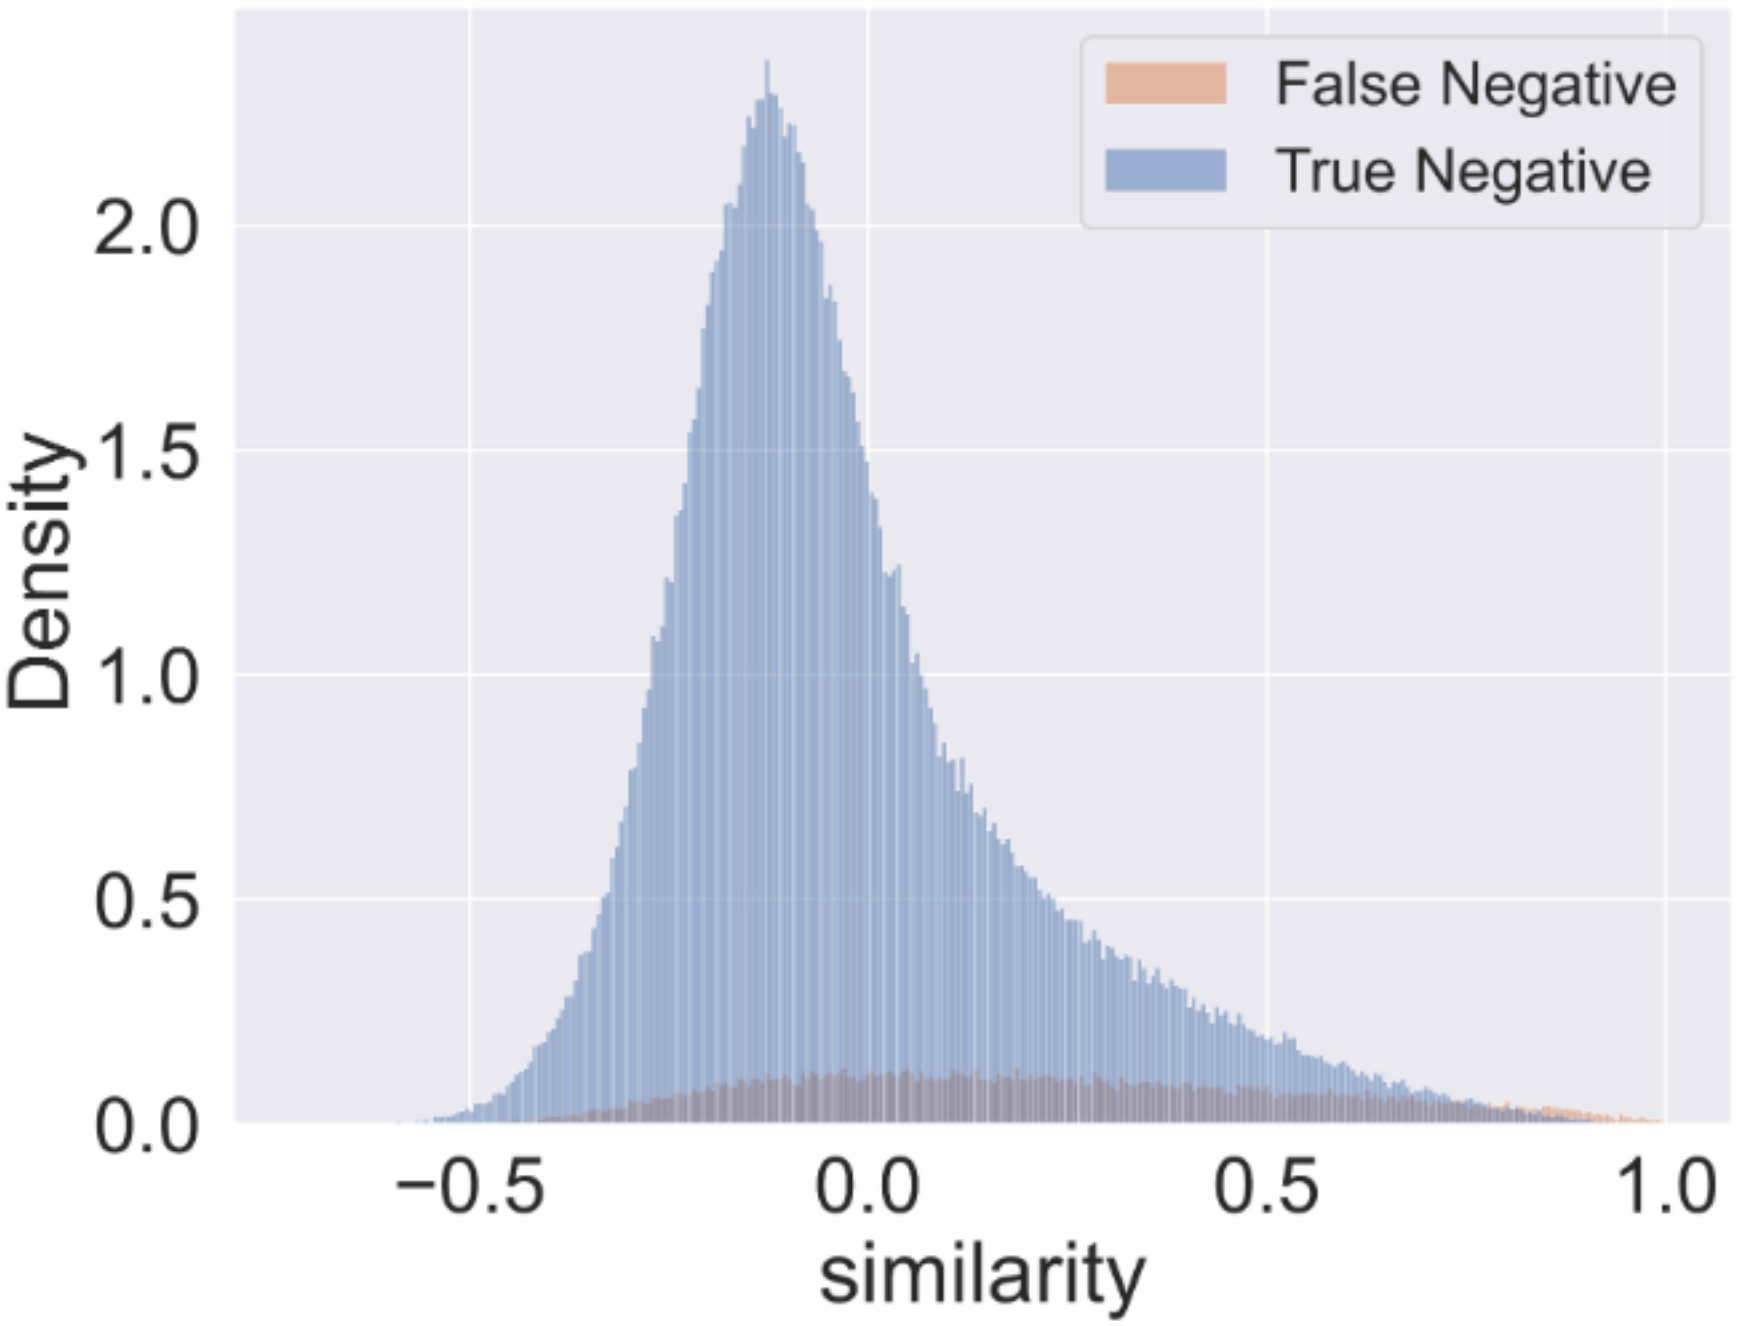
\includegraphics[width=4.8cm]{images/sim_negatives_image_data.png} }}%
    \qquad
    \subfloat[\centering Coauthor-CS (Graph). Most similar negative samples are \acp{fn}.]
    {{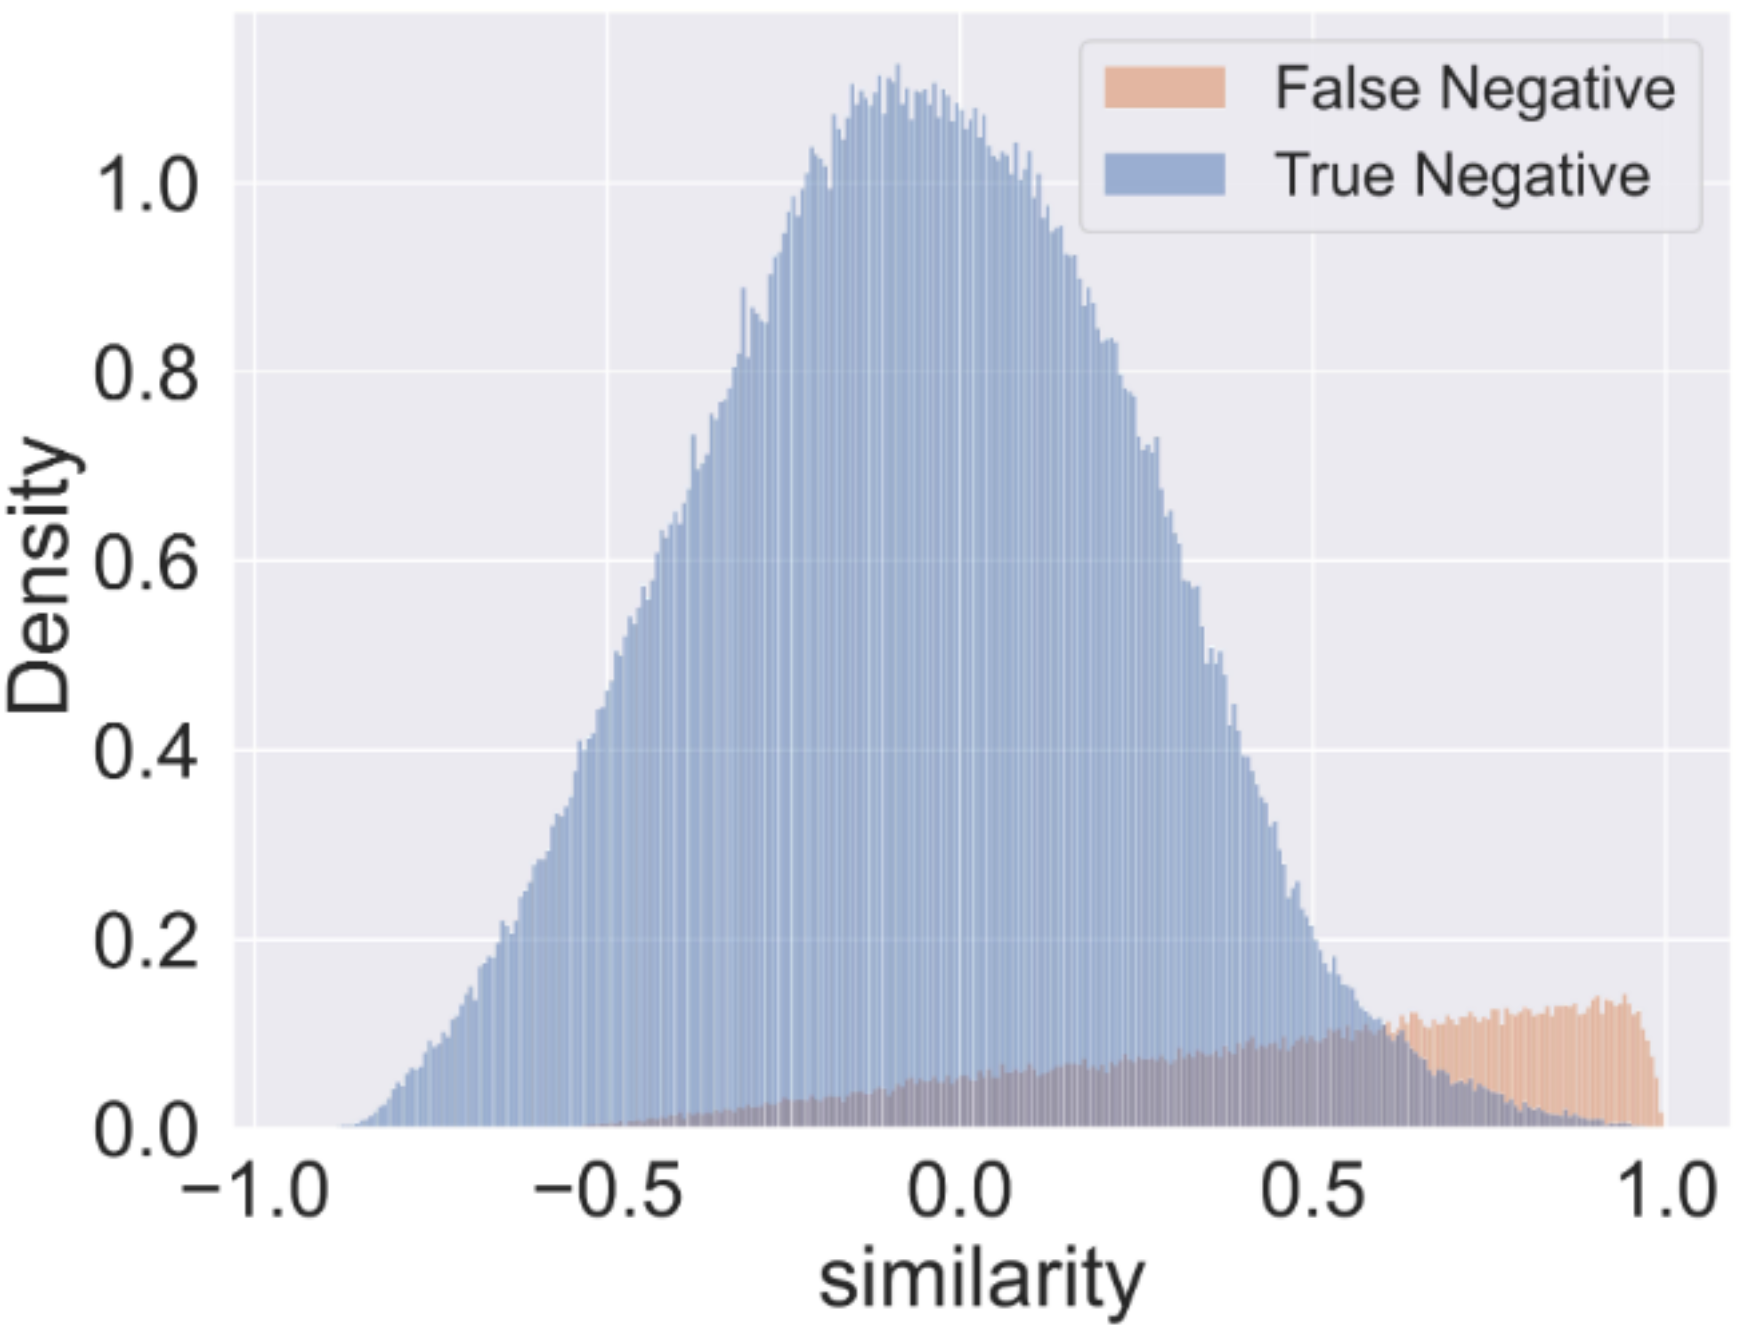
\includegraphics[width=5.2cm]{images/sim_negatives_graph_data.png} }}%
    \caption{Histogram of similarity between anchor and negative samples for \ac{cl} and \ac{gcl} from \citet{progcl_2022}.
    Blue denotes the empirical distribution of the \acp{tn}, while orange denotes \acp{fn}.}%
    \label{fig:sim_t_f_neg_image_graph}%
\end{figure}

% scheme 1: ProGCL-weight
Based on this observation, the first approach the authors propose is considering a combination of the probability of a sample being a \ac{tn} 
with the sample's similarity to the anchor, i.e. its hardness, during the selection process of negative samples.

% scheme 2: ProGCL-mix (MoCHi)
\begin{equation}
    \tilde{h_k} =  \alpha_k \cdot n_i + (1-\alpha_k) \cdot  n_j, \text{ where } \alpha_k = \frac{p(n_i \text{ is } TP)}{p(n_i \text{ is } TP) + p(n_j \text{ is } TP)}
    \label{eq:progcl_mix}
\end{equation}

Furthermore, the authors present an extension of the hard mining strategy \ac{mochi} introduced in \autoref{subsec:MoCHi}.
They claim, that a high portion of the negative samples generated by \ac{mochi} are \acp{fn}.
They therefore propose to weigh the selected negative samples for mixing 
according to their relative probability of being a \ac{tn} as displayed in \Eqref{eq:progcl_mix}.

